\chapter{Background}

In this chapter, we explore the current research on this topic. First, by exploring the theory behind liquid neural networks, in comparison to deep neural networks. Then, by investigating current verification methods and assessing their suitability to liquid neural networks. The reader should have an understanding of (traditional) neural networks and linear algebra concepts.

\section{Liquid Neural Networks}

Liquid neural networks, introduced by Ramin Hasani et al. (2021) \cite{hasaniLiquidTimeconstantNetworks2021}, are a novel class of AI algorithms, designed to maintain adaptability after completing training. These are inspired by the communication patterns of brain cells, which are flexible and responsive to new/unseen data even after their initial training phase. 

Traditional neural networks use fixed architectures and static parameters, so require retraining to handle new information. Liquid neural networks use \textbf{continuous-time dynamics} to enable their state to evolve smoothly over time. This means they can dynamically adjust their responses to changing inputs during inference. This structure allows these networks to be robust against perturbations and capable of generating complex behaviors without requiring large-scale architectures.

LNNs use differential equations to simulate the continuous/dynamic processing and plasticity of the brain. Since LNN neurons communicate selectively with a subset of other neurons, connections formed are sparse (unlike traditional deep neural networks with dense fully-connected layers). This makes LNNs more computationally efficient than deep neural networks.

There are a range of applications of LNNs. Hasani suggests that their inherent adaptability makes them suitable for tasks requiring real-time learning and decision-making, such as autonomous driving and medical diagnosis. Their efficiency could address several challenges associated with large-scale machine learning systems, including issues related to interpretability, accountability, and environmental impact due to high carbon footprints. \cite{tedxtalksLiquidNeuralNetworks2023}

\subsection{Continuous-Time Dynamical Systems/Differential Equations}

A \textbf{continuous-time dynamical system} is a mathematical model used to describe a system that evolves over time in a way that is continuous (rather than discrete). This means the state of the system changes smoothly as a function of time, without abrupt jumps.

In the context of liquid neural networks, the neurons' states evolve as continuous-time dynamical systems. Each neuron’s state is governed by \textbf{differential equations}, enabling the network to process information dynamically and adaptively, much like physical systems in the real world. This is inspired by biological neurons, where the activity of each neuron is influenced dynamically by inputs and changes over time.

The state of each neuron \(x_i(t)\) in an LNN evolves over time according to a differential equation, expressed as:

\begin{equation} \label{eq:1}
    \frac{dx_i(t)}{dt} = f(x_i(t), u_i(t), t; \theta_i),
    \end{equation}

where:
\begin{itemize}
    \item \(x_i(t)\): The internal state of the \(i\)-th neuron at time \(t\),
    \item \(u_i(t)\): The input signal to the \(i\)-th neuron at time \(t\),
    \item \(t\): Time, treated as a continuous variable,
    \item \(\theta_i\): Trainable parameters of the neuron, such as weights and biases,
    \item \(f(\cdot)\): A function (usually nonlinear) describing the neuron’s dynamics.
\end{itemize}

A common differential equation is the \textbf{leaky integrator dynamics}, where the state evolves as:
\[
\frac{dx_i(t)}{dt} = -\alpha x_i(t) + \sum_{j=1}^N w_{ij} h(x_j(t)) + u_i(t),
\]
with:
\begin{itemize}
    \item \(-\alpha x_i(t)\): A "leakage" term causing the neuron’s state to decay over time, with \(\alpha > 0\) representing the decay rate (temporal decay),
    \item \(\sum_{j=1}^N w_{ij} h(x_j(t))\): The weighted input from other neurons, where \(w_{ij}\) is the weight from neuron \(j\) to \(i\), and \(h(x_j(t))\) is a nonlinear activation function (e.g., \(\tanh\) or ReLU),
    \item \(u_i(t)\): An external input signal.
\end{itemize}

For more complex systems, \textbf{nonlinear terms} can be included, resulting in equations such as:
\[
\frac{dx_i(t)}{dt} = g(x_i(t)) + \sum_{j=1}^N w_{ij} \sigma(x_j(t)) + u_i(t),
\]
where \(g(x_i(t))\) models intrinsic nonlinear dynamics, and \(\sigma(x_j(t))\) is a nonlinear activation function.

A liquid neural network, as a continuous-time dynamical system, has several important features. First, it ensures \textbf{smooth evolution}, where the neuron states evolve continuously over time according to differential equations. This smooth state transition is essential for modeling time-dependent values in tasks like time-series forecasting or control systems. In addition, the dynamics of the network incorporate \textbf{time dependency} \(t\) explicitly or depend solely on the current state \(x(t)\), enabling the network to capture both static and dynamic temporal relationships. Liquid neural networks are also typically \textbf{deterministic}, with their future states fully defined by the current states and inputs, but they can also accommodate \textbf{stochastic elements} to model uncertainty or noise in the environment. Finally, the network may operate under \textbf{linear} dynamics, such as \(f(x) = Ax + Bu\), which are efficient but limited in complexity, or \textbf{nonlinear} dynamics, like \(f(x) = \tanh(Wx + b)\), which allow the network to represent intricate patterns and adaptive behaviours.

\subsection{LNN Training}
During training, the above differential equations (\ref{eq:1}) define how each neurons processes information. For each labelled training data sample, the following process occurs.

During the \textbf{forward pass}, the system of differential equations is numerically solved over time, starting from an initial state \(x(0)\). Inputs \(u(t)\) and parameters \(\theta_i\) drive the evolution of neuron states \(x_i(t)\).

The network then outputs a value, derived from the neuron states. This is compared to the target output to compute a \textbf{loss function}.

During \textbf{backpropagation through time}, gradients of the loss with respect to trainable parameters (\(\theta_i\)) are computed by differentiating through the differential equations using methods like automatic differentiation or adjoint sensitivity analysis.

Finally, \textbf{optimization algorithms} (e.g. gradient descent) update the parameters of the DEs to minimize the loss.

\subsection{LNN Inference}
During inference, the same differential equations govern the neuron states, but parameters (\(\theta_i\)) are fixed. The network processes dynamic inputs \(u(t)\) in real-time. The equation also considers the neuron's previous state \(x_i(t)\), which is dependent on previous input values \(u(t)\). Thus, the output of each neuron is dependent on the parameters, current input values, and previously seen input values.

\subsection{Advantages of LNNs}
Using differential equations in LNNs provides several advantages.
\subsubsection{Temporal Modelling}
Continuous dynamics are well-suited for time-dependent tasks. This means LNNs can be used to find time-based relationships in data (temporal modeling). This form of 'memory' is highly beneficial in time-series tasks.

The nonlinear nature of \(f(x_i(t))\) ensures that the network captures complex temporal dependencies, allowing it to adjust its behavior based on the sequence and timing of inputs. This dynamic capability provides the network with a form of memory, enabling it to adapt to new scenarios even outside the training set.

This is in contrast to static models which consider data points to be independent and identically distributed.

\subsubsection{Adaptability}
Dynamic state evolution allows the network to adapt during deployment.

The differential equation model (\ref{eq:1}) for liquid neural networks allows for state evolution even after training, resulting in increased adaptability. This is achieved by the continuous dynamics governing neuron states, which enable the network to respond dynamically to real-time inputs and changing environments.

In the DE model, \(x_i(t)\) is the state of the \(i\)-th neuron at time \(t\), \(u_i(t)\) represents external inputs, \(t\) is time, and \(\theta_i\) are trainable parameters (e.g., weights and biases). After training, the parameters \(\theta_i\) are fixed, but the neuron states \(x_i(t)\) continue to respond dynamically to new inputs \(u_i(t)\). This means the network integrates real-time inputs into its state over time, adapting its behavior dynamically to variations in the input patterns or the timing of events.

The differential equations governing the states ensure that even small variations in the input influence the system, enabling real-time adaptation.

This provides several advantages. LNNs excel in real-world scenarios involving dynamic environments, such as robotics \cite{chahineRobustFlightNavigation2023} and control systems.

For example, an LNN controlling a robotic arm in a dynamic environment would learn general principles of motion and control during training. During inference, as new obstacles appear or external forces are applied, the network integrates this new information into its state \(x_i(t)\) dynamically. This allows the robotic arm to adjust its movements in real time without needing retraining for each specific scenario.

In addition, by dynamically evolving its states, the network generalizes better to unseen data patterns by interpolating between learned behaviors.

\subsubsection{Efficiency}
Liquid neural networks (LNNs) are inherently more efficient than traditional deep neural networks (DNNs) due to their ability to maintain sparser representations. At any given time, only a subset of an LNNs' neurons or parameters are significantly active or contribute to the system's computations. This sparsity reduces the computational overhead while retaining the network's performance and adaptability.

This is because continuous-time dynamics favor selective activity. In LNNs, neuron states evolved continuously over time, according to the differential equation \ref{eq:1}. Here \(f(\cdot)\) determines how each neuron state changes based on its inputs, past states, and parameters. The use of continuous-time dynamics enables neurons to become active only when relevant input signals \(u_i(t)\) or temporal events trigger them. This selective activity leads to fewer neurons being active at a given time, resulting in sparse representations.

LNNs are designed to work efficiently with fewer parameters compared to DNNs. While in traditional DNNs, layers are often densely connected, meaning all neurons in one layer interact with all neurons in the next layer. LNNs use sparse connectivity patterns, where neurons only interact with a limited subset of other neurons. This reflects real-world systems, such as biological brains, where neurons form selective, sparse connections.The sparsity of connections reduces the number of computations required during both training and inference.

LNNs allow the internal states of neurons to evolve over time and depend on the dynamics of the inputs. Because of this adaptability, only neurons relevant to the current input remain active. This reduces unnecessary computations and avoids the inefficiencies of global activation in traditional DNNs.

The continuous dynamics of LNNs inherently encode temporal dependencies. Unlike recurrent neural networks (RNNs) or deep learning models that require explicit mechanisms like memory gates (e.g., in LSTMs or GRUs), LNNs rely on the fluid evolution of neuron states. This reduces the overhead of managing and updating memory states, further contributing to sparsity and efficiency.

The sparse nature of LNNs offers several advantages over traditional DNNs, including reduced computational cost (minimizing matrix operations), lower energy consumption, better scalability, and robustness to overfitting (as sparse connectivity can act as a regularization mechanism by ensuring only essential features are focussed on).

\subsubsection{Stability}
LNNs exhibit greater stability and robustness to noise compared to traditional DNNs. 

Continuous time dynamics and differential equations encode stability constraints, ensuring smooth transitions between states.

In LNNs, the state of each neuron evolves over time according to the differential equation \ref{eq:1}. The continuous nature of these equations ensures that the neuron states change gradually over time. As a result, sudden spikes in the input \(u_i(t)\) (caused by noise) are naturally smoothed out. This gradual evolution prevents abrupt changes in the neuron states, making the network less sensitive to transient noise.

In addition, neuron states evolve in response to both the current input \(u_i(t)\) and past states \(x_i(t)\). This integration over time allows the network to prioritize long-term patterns in the input and ignore temporary noise. The feedback from past states enables temporal filtering, where only meaningful input changes accumulate and influence the network’s output. In contrast, the layer-by-layer static activations in DNNs make them more susceptible to noise.

In traditional DNNs, noisy inputs can propagate through the network, often being amplified by dense connections and static parameter updates. To avoid this, special techniques can be used such as dropout. However, LNNs achieve this implicitly, by using sparse and selective connections. This limits the propagation of noise across the network. The continuous evolution of states ensures that transient noise does not significantly affect downstream neurons or outputs.

This enhanced stability has a range of benefits. LNNs perform well in real-world settings where inputs are often corrupted. The intrinsic smoothing abilities of LNNs also reduces the amount of noise-filtering preprocessing required.

\section{Neural Network Verification}

In this section we explore the problem of neural network verification. We look at current methods used for DNN verification, which will form the inspiration for a liquid neural network verification approach. The suitability of these to LNNs must be evaluated.

\subsection{The Verification Problem}

Verification problems can involve concrete bounds on the input and linear programming (LP) constraints on the output. Formally, the problem can be defined as follows:

\textbf{Definition 2.2.1.1} Let \( f : \mathbb{R}^n \to \mathbb{R}^m \) be a neural network, and let \( \mathcal{X} = \{x' \in \mathbb{R}^n \mid x_i^l \leq x_i' \leq x_i^u \} \) represent the set of valid inputs constrained by the lower and upper bounds \(x^l, x^u\). Given a set of linear constraints on the output \( \psi_y \), let \( \mathcal{Y} = \{ y \mid \psi_y \} \) denote the set of outputs satisfying \( \psi_y \). The verification problem is to determine whether \( x' \in \mathcal{X} \implies f(x') \in \mathcal{Y} \), or to find a counterexample \( x' \in \mathcal{X} \) such that this implication is not true. \label{verification_def}

For input and output constraints as defined above, the goal is either to prove that no valid input violates the output constraints or to find an input that does. If no input satisfies the output constraints, we declare the property as ``safe.'' Otherwise, if such an input exists, the property is deemed ``unsafe,'' and the corresponding input serves as a counterexample. \cite {henriksenEfficientNeuralNetwork}


\subsection{Motivation}

Verification of neural networks is a crucial problem, especially when a new architecture (such as liquid neural networks) is being researched. This is because neural networks are often deployed in safety-critical applications, such as autonomous vehicles or medical diagnosis, where unpredictability can cause significant harm. Neural networks are also vulnerable to adversarial attacks, which is when small perturbations within input data (often unnoticable to the human eye) cause significant undesired changes in the output. This vulnerability poses a serious threat to their reliability and trustworthiness. Verification ensures that the network behaves as expected under specified conditions, whilst robustness verification focuses on guaranteeing that small perturbations in the input do not lead to misclassifications or unsafe behavior. By formally proving properties of neural networks or identifying counterexamples, verification helps to ensure safety and mitigate risks in real-world deployments.

\subsection{Recurrent Neural Networks}

We now focus on the verification problem in relation to recurrent neural networks (RNNs) specifically. RNNs are deep neural networks trained on sequential or time series data to create a model that can make sequential predictions or conclusions based on sequential inputs. During both training and inference, they also use information from prior inputs to influence the current input and output. In traditional recurrent neural networks, this is achieved by a feedback loop within the network, containing a hidden state which 'remembers' previous inputs. \cite{WhatRecurrentNeural2021}

\begin{figure}[h!]
    \centering
    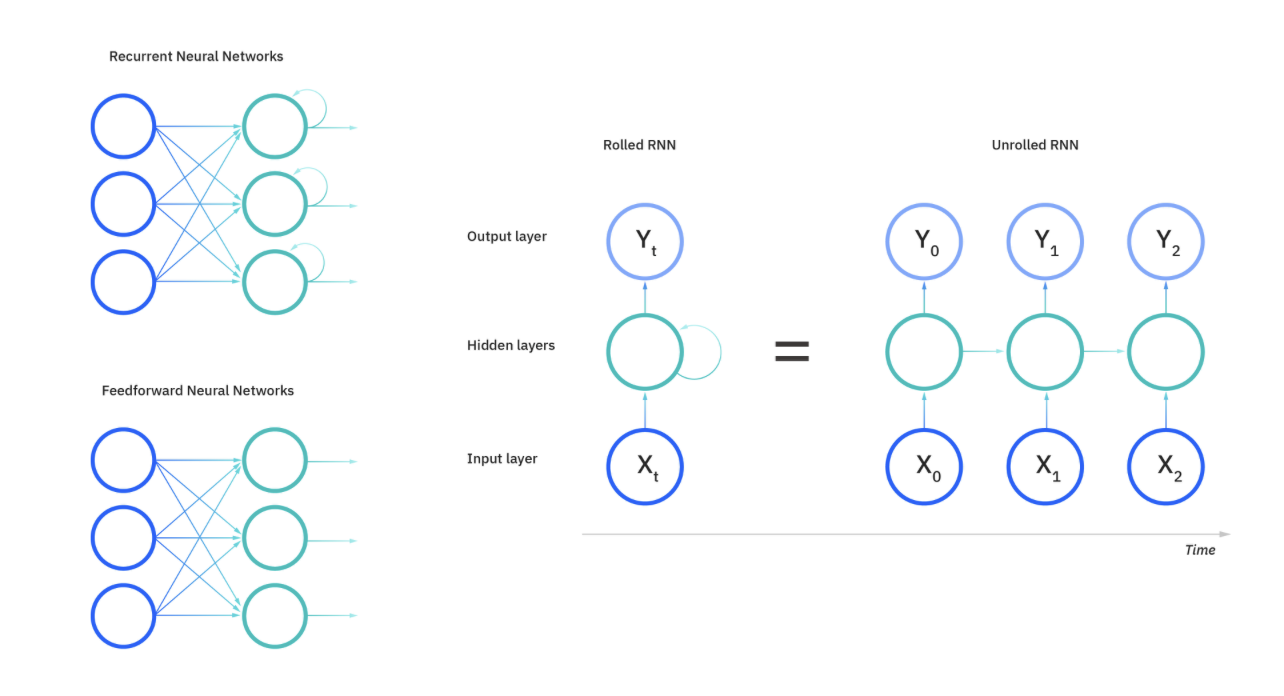
\includegraphics[width=0.8\textwidth]{images/RNN_vs_FeedForward.png}
    \caption{Feedforward (traditional) vs. Recurrent Neural Networks}
    \label{fig:example_image}
\end{figure}

RNNs rely on Backpropagation Through Time (BPTT) to compute gradients, unlike traditional neural networks that use standard backpropagation. Whilst BPTT follows the same principles as traditional methods, adjusting parameters by propagating errors from output to input layers, it accounts for sequential data by summing errors across time steps. This temporal error accumulation differentiates BPTT from the simpler gradient computation in feedforward networks, which lack a time-dependent structure.

'Memory' in RNNs can be achieved by several architectures, such as LSTM (Long Short-Term Memory), GRU (Gated Recurrent Units) and Encoder-decoder RNNs. Since liquid neural networks leverage differential equations to achieve a form of 'memory', they are a specialized type of RNN. Whilst their weights are typically fixed, the hidden state evolves dynamically over time, driven by the structure of the differential equations and the input. This continuous evolution allows liquid networks to retain memory and capture temporal dependencies across varying time scales.

The verification problem for RNNs involve constraints on both the input sequences and the dynamic outputs of the network, with the goal of solving the problem stated earlier (\ref{verification_def}). This requires handling both the sequence-based inputs and the time-evolving hidden states.

\subsection{Robustness Verification for Recurrent Neural Networks}

An important verification problem for RNNs concerns their robustness to temporal perturbations or noise in sequential inputs. Robustness implies that small perturbations in the input sequence do not cause significant deviations in the network's output. This can be formalized as follows:

\textbf{Definition 2.2.4.1.} Let \( x \in \mathbb{R}^n \) be a sequential input to a recurrent neural network \( f : \mathbb{R}^n \to \mathbb{R}^m \), where \( m > 1 \) represents the dimensionality of the output space. Let \( \mathcal{C}_x = \{ x' \in \mathbb{R}^n \mid x_i^l \leq x_i' \leq x_i^u \} \) represent the set of perturbed input sequences. The \textit{targeted robustness verification problem} is to determine whether
\[
x' \in \mathcal{C}_x \implies f(x')_c > f(x')_t \quad \text{for a specific output target } t,
\]
or to find a counterexample \( x' \) such that this implication is not satisfied.

\textbf{Definition 2.2.4.2} Let \( x \in \mathbb{R}^n \) be a sequential input to a recurrent neural network \( f : \mathbb{R}^n \to \mathbb{R}^m \), where \( m > 1 \). Let \( \mathcal{C}_x = \{ x' \in \mathbb{R}^n \mid x_i^l \leq x_i' \leq x_i^u \} \). The \textit{general robustness verification problem} is to determine whether
\[
x' \in \mathcal{C}_x \implies f(x')_c > f(x')_t \quad \text{for all } t \neq c,
\]
or to find a counterexample \( x' \) where this implication fails.

Robustness verification for RNNs focuses on ensuring that temporal variations in sequential inputs do not cause undesired behavior. Specifically, the targeted robustness problem can often be reduced to verifying specific temporal constraints or perturbations in the input sequence. The general robustness problem is more challenging because it involves verifying the network's behavior across all possible perturbations and output dimensions. These problems may require advanced techniques, which will be discussed in the following sections.

\subsection{Symbolic and Interval Propagation Methods}

This section explores methods that focus on propagating bounds through liquid neural networks, which verifies their robustness when faced with input perturbations. \textbf{Symbolic Interval Propagation (SIP)} is a technique that computes conservative output bounds using interval arithmetic, providing a computationally efficient way to check for robustness. \textbf{CROWN (Certified Robustness to Weight Perturbations)} is more complex, and introduces linear approximations which improves the precision of robustness verification. \textbf{Lipschitz-based methods} they estimate global sensitivity by bounding the Lipschitz constant of the network. These approaches are particularly useful for ensuring scalability and efficiency, making them suitable for applications where lightweight and real-time verification is required.

\subsubsection{SIP (Symbolic Interval Propagation)}

SIP is a scalable and efficient technique for verifying liquid neural networks by propagating symbolic intervals through the layers of the network to bound the range of possible outputs. For LNNs governed by neural ODEs with the equation \ref{eq:1}, SIP can be applied to discretize and propagate bounds over time, handling non-linearity and ensuring robustness and safety properties are satisfied under perturbations.

\paragraph{Steps in SIP:}
\begin{enumerate}
    \item \textbf{Input Interval Initialization}:
    Define the input range as intervals \([l_i, u_i]\) for each dimension \(x_i\), forming a hyper-rectangle. These intervals are represented symbolically to maintain dependencies between variables.
    
    \item \textbf{Symbolic Propagation Through Layers}:
    At each discretized time step or layer:
    \begin{itemize}
        \item \textbf{Affine Transformations}:
        For a layer \(z = W x + b\), bounds are propagated symbolically:
        \[
        l_z = W \cdot l_x + b, \quad u_z = W \cdot u_x + b.
        \]
        \item \textbf{Nonlinear Activations}:
        Nonlinearities like ReLU or \(\tanh\) are handled by updating bounds:
        \[
        \text{ReLU: } [\max(0, l_z), \max(0, u_z)], \quad
        \text{Tanh: } [\tanh(l_z), \tanh(u_z)].
        \]
    \end{itemize}
    
    \item \textbf{Output Interval Verification}:
    The final output intervals are compared against safety or robustness properties. For example, given input perturbations \(\delta x\), the output bounds \(F(x)\) must satisfy:
    \[
    F(x + \delta x) \subseteq [F_L, F_U],
    \]
    where \(F_L\) and \(F_U\) are symbolic bounds on the output.
\end{enumerate}

\paragraph{Advantages for Liquid Neural Networks}
SIP is well-suited for LNNs due to its ability to handle the continuous evolution of states in neural ODEs:
\begin{itemize}
    \item Precision: Symbolic intervals maintain variable dependencies, producing tighter bounds than traditional interval arithmetic.
    \item Efficiency: Propagation avoids the computational cost of exact methods, making SIP scalable for larger networks.
    \item Adaptability: SIP can handle nonlinear dynamics in LNNs through accurate approximations of activation functions.
\end{itemize}

\paragraph{Practical Considerations}
One consideration is over-approximation - accumulated conservativeness may reduce precision in deeper networks. Also, complex nonlinearities (within highly nonlinear layers such as softmax) require additional approximations, introducing potential conservatism. Finally, for neural ODEs, time discretization must balance accuracy with computational cost.

\subsubsection{CROWN (Certified Robustness to Weight Perturbations)}

CROWN (Certified Robustness to Weight Perturbations) is a general framework for certifying the robustness of neural networks, including those with non-linear activation functions. It achieves this by bounding the outputs of the network using adaptive linear (or quadratic) upper and lower bounds for each activation function. For liquid neural networks, governed by neural ODEs, CROWN can be adapted to certify robustness by discretizing the continuous dynamics and applying its bounding technique to each time step.

CROWN provides an efficient and scalable method for verifying the robustness of LNNs. The propagated adapted bounds ensure that perturbations in the input do not lead to significant deviations in the output.

\paragraph{Mathematical Framework}
Consider a liquid neural network modeled as:
\[
\frac{dx(t)}{dt} = f(x(t), t, \theta),
\]
where \(x(t) \in \mathbb{R}^n\) is the state, \(f(x, t, \theta)\) describes the dynamics, and \(\theta\) represents the parameters. For a given perturbed input \(x_0 \in \mathbb{R}^n\) within an \(\ell_p\)-ball:
\[
x \in B_p(x_0, \epsilon) = \{x \mid \|x - x_0\|_p \leq \epsilon\},
\]
CROWN aims to compute certified bounds \(F_L(x) \leq F(x) \leq F_U(x)\), where \(F(x)\) is the output of the neural ODE after a fixed time horizon \(T\).

\paragraph{Bounding Nonlinearities}
For each activation function \(\sigma(y)\), CROWN constructs linear upper and lower bounds:
\[
h_U(y) = \alpha_U y + \beta_U, \quad h_L(y) = \alpha_L y + \beta_L,
\]
such that \(h_L(y) \leq \sigma(y) \leq h_U(y)\) over a pre-activation range \([l, u]\). These bounds are propagated through the layers of the network. For LNNs, this involves discretizing the time domain into intervals \([t_k, t_{k+1}]\) and applying the bounds iteratively at each time step.

\paragraph{Output Certification}
To certify robustness, CROWN computes bounds on the network's output \(F(x)\). Using the layer-by-layer propagation of the upper and lower bounds, the output bounds are expressed as:
\[
F_U(x) = \Lambda^{(0)} x + \sum_{k=1}^m \Lambda^{(k)} (b^{(k)} + \Delta^{(k)}), \quad
F_L(x) = \Omega^{(0)} x + \sum_{k=1}^m \Omega^{(k)} (b^{(k)} + \Theta^{(k)}),
\]
where \(\Lambda\) and \(\Omega\) are matrices representing the upper and lower bound propagation, and \(\Delta\) and \(\Theta\) account for biases introduced by non-linearities.

\paragraph{Application to Neural ODEs}
For neural ODEs, the propagation framework is adapted to account for the continuous evolution of states. The bounds are computed at each discretized step \(t_k\), ensuring that the dynamics satisfy the robustness conditions:
\[
F_U(x_0) - F_L(x_0) \geq \delta,
\]
where \(\delta\) is the minimum required margin for robustness.

\paragraph{Practical Implementation}
CROWN can be implemented as follows:
\begin{enumerate}
    \item \textbf{Define Input Bounds}: Specify the \(\ell_p\)-ball around the input \(x_0\) and initialize the pre-activation bounds for the first layer.
    \item \textbf{Propagate Bounds}: Compute the upper and lower bounds layer-by-layer using the adaptive linear approximations.
    \item \textbf{Certify Robustness}: Verify that the certified bounds at the output satisfy the desired robustness property (e.g., consistent classification).
\end{enumerate}
\cite{zhangEfficientNeuralNetwork2018}

\subsubsection{Lipschitz-Based Methods}

Lipschitz-based methods provide a robust framework for verifying the safety and robustness of liquid neural networks by quantifying how sensitive a network's outputs are to perturbations in its inputs. Their ability to provide global robustness guarantees is useful for neural ODEs. The Lipschitz constant of a network bounds the maximum rate at which outputs can change with respect to changes in inputs, ensuring that small input perturbations do not lead to large deviations in the output.

\paragraph{Mathematical Foundation}
For a liquid neural network modeled as:
\[
\frac{dx(t)}{dt} = f(x(t), t, \theta),
\]
where \(x(t) \in \mathbb{R}^n\) is the state, \(f(x, t, \theta)\) defines the dynamics, and \(\theta\) are the network parameters, the Lipschitz constant \(L\) satisfies:
\[
\|F(x) - F(y)\| \leq L \|x - y\|, \quad \forall x, y \in \mathbb{R}^n,
\]
where \(F(x)\) represents the solution to the neural ODE at the final time \(T\). The Lipschitz constant \(L\) bounds the global sensitivity of the network.

\paragraph{Estimation of the Lipschitz Constant}
The Lipschitz constant can be estimated for an LNN by analyzing the Jacobian of \(f(x, t, \theta)\). For a time-discretized system, the sensitivity of the network is determined by:
\[
L = \sup_{t \in [0, T]} \| J_f(x, t) \|,
\]
where \(J_f(x, t) = \frac{\partial f(x, t, \theta)}{\partial x}\) is the Jacobian matrix of \(f\). Computing or bounding \(L\) involves:
\begin{itemize}
    \item \textbf{Spectral Norm Analysis}: Evaluating \(\|J_f(x, t)\|\) as the largest singular value of the Jacobian at each time step.
    \item \textbf{Pathwise Integral Bounds}: For neural ODEs, \(L\) can be bounded using the integral of the Jacobian along the trajectory:
    \[
    L \leq \int_0^T \|J_f(x(t), t)\| dt.
    \]
\end{itemize}

\paragraph{Verification Applications}
Lipschitz-based methods are widely used for:
\begin{enumerate}
    \item \textbf{Robustness Verification}: Verifying that small input perturbations \(x_0 \to x_0 + \delta x\) result in bounded output deviations, ensuring:
    \[
    \|F(x_0 + \delta x) - F(x_0)\| \leq L \|\delta x\|.
    \]
    \item \textbf{Safety Analysis}: Ensuring the network’s outputs remain within a safe region under bounded input perturbations.
    \item \textbf{Adversarial Robustness}: Certifying that adversarial inputs cannot change the classification or decision boundaries within a certain radius.
\end{enumerate}

\paragraph{Practical Implementation}
To implement Lipschitz-based verification for LNNs:
\begin{enumerate}
    \item \textbf{Compute the Lipschitz Constant}: Use numerical methods, such as spectral norm approximation or pathwise integration, to estimate \(L\).
    \item \textbf{Bound Output Sensitivity}: Evaluate \(L\) for given input perturbations \(\delta x\) and verify that the resulting outputs satisfy safety and robustness criteria.
    \item \textbf{Scaling for Efficiency}: For high-dimensional networks, consider approximation techniques or layer-wise bounds to improve scalability.
\end{enumerate}

\subsection{Optimisation-Based Verification}

This section focuses on verification methods that rely on optimization to certify the safety, stability, or robustness of liquid neural networks. \textbf{Mixed Integer Linear Programming (MILP)} solvers reframe verification as a constrained optimization problem, allowing exact solutions that guarantee robustness against adversarial perturbations or input variability. \textbf{POPQORN (Quantifying Robustness of Recurrent Neural Networks)} takes a  probabilistic approach to quantify robustness whilst maintaining computational efficiency, making it suitable for larger and more complex networks. \textbf{Control Barrier Functions (CBFs)} provide safety assurances by optimizing control policies to keep system trajectories within predefined safe regions. These methods are useful for high-precision situations such as robotics or automation systems.


\subsubsection{Mixed Integer Linear Programming (MILP) Solver for RNNs}

MILP provides a rigorous framework for verifying liquid neural networks, modeled by neural ODEs. By discretizing continuous dynamics and formulating verification as linear constraints with integer variables, MILP ensures exact guarantees for robustness and safety properties.

\paragraph{Formulating the MILP Problem}
For an LNN described by:
\[
\frac{dx(t)}{dt} = f(x(t), t, \theta),
\]
where \(x(t) \in \mathbb{R}^n\) is the state and \(f(x, t, \theta)\) defines the dynamics, MILP discretizes the time domain into intervals \([t_k, t_{k+1}]\), approximating the dynamics as:
\[
x_{k+1} = x_k + \Delta t \cdot f(x_k, t_k, \theta),
\]
where \(\Delta t\) is the time step. Nonlinear activation functions (e.g., \(\sigma(\cdot)\), \(\tanh(\cdot)\)) are linearized using binary variables, enabling a mixed-integer formulation.

\paragraph{Verification via Constraints}
MILP verifies robustness by ensuring that output properties hold under input perturbations. For an input \(x_0\) perturbed within:
\[
x_0 \in B_p(x_0, \epsilon) = \{x \mid \|x - x_0\|_p \leq \epsilon\},
\]
the output \(F(X)\) must satisfy:
\[
F_j(X) \geq F_i(X), \quad \forall i \neq j,
\]
where \(j\) is the correct label. This is encoded as linear constraints, ensuring that adversarial inputs do not cause misclassification.

\paragraph{Optimization Structure}
The MILP problem includes:
\begin{itemize}
    \item Objective Function:
    \[
    \max_\epsilon \epsilon, \quad \text{subject to constraints}.
    \]
    \item Linear Constraints: Enforce dynamics:
    \[
    x_{k+1} = x_k + \Delta t \cdot f(x_k, t_k, \theta),
    \]
    and robustness:
    \[
    F_j(X) \geq F_i(X), \quad \forall i \neq j.
    \]
    \item Binary Variables: Handle nonlinear activations or branching decisions.
\end{itemize}

\paragraph{Applications and Limitations}
MILP is particularly effective for verifying robustness, safety, and stability in LNNs under bounded uncertainties. However, its computational complexity grows with the network size and time steps. Techniques such as constraint relaxation and parallel solvers mitigate these challenges, making MILP viable for moderately sized networks.

\paragraph{Conclusion}
MILP offers exact verification by translating neural ODE dynamics into mixed-integer constraints. This approach is invaluable for ensuring robustness and safety in liquid neural networks, particularly in safety-critical applications. \cite{xueRNNBasedFrameworkMILP2023}

\subsubsection{POPQORN (Quantifying Robustness of Recurrent Neural Networks)}

POPQORN verifies robustness of RNNs under adversarial perturbations by bounding a network's output using linear functions. It ensures certified output bounds, making it valuable for safety-critical applications where adversarial robustness is essential. For liquid neural networks, modeled by:
\[
\frac{dx(t)}{dt} = f(x(t), t, \theta),
\]
POPQORN computes certified bounds on the output \(F(X)\) when inputs \(X\) are perturbed within an \(\ell_p\)-norm ball:
\[
x(k) \in B_p(x(k)_0, \epsilon),
\]
where \(B_p(x(k)_0, \epsilon) = \{x \mid \|x - x(k)_0\|_p \leq \epsilon\}\). The output is bounded as:
\[
F_L(X) \leq F(X) \leq F_U(X),
\]
with \(F_L(X)\) and \(F_U(X)\) propagated backward through the network.

\paragraph{Handling Nonlinearities}
Nonlinear activation functions, such as \(\sigma(\cdot)\) or \(\tanh(\cdot)\), are bounded by linear approximations:
\[
h_U(v) = \alpha_U v + \beta_U, \quad h_L(v) = \alpha_L v + \beta_L,
\]
such that \(h_L(v) \leq \sigma(v) \leq h_U(v)\) over a pre-activation range \([l, u]\). These linear bounds are propagated recursively, capturing the effects of nonlinearity.

\paragraph{Robustness Optimization}
POPQORN formulates robustness verification as an optimization problem to find the largest perturbation \(\epsilon\) that preserves the predicted label \(j\):
\[
\epsilon_j = \max_\epsilon \, \epsilon, \quad \text{subject to } F_L^j(X) \geq F_U^i(X), \, \forall i \neq j.
\]
This ensures the network remains robust to adversarial inputs within the certified bounds.

\paragraph{Application and Practical Steps}
For LNNs, POPQORN adapts to continuous dynamics by discretizing time steps and applying bounds iteratively:
\[
F_j(X) = \int_0^T W(t)x(t) \, dt + b.
\]
Key steps include pre-activation bound computation, recursive linear propagation, and solving the optimization problem via binary search. Experimental results demonstrate its efficacy for quantifying robustness in RNNs, extendable to neural ODEs. \cite{koPOPQORNQuantifyingRobustness2019}

\subsubsection{Control Barrier Functions (CBFs)}

Control Barrier Functions (CBFs) provide a powerful optimization-based framework for verifying the safety and stability of liquid neural networks (LNNs) in real-time, modeled by neural ordinary differential equations (ODEs). A CBF \(h(x): \mathbb{R}^n \to \mathbb{R}\) defines a safe set:
\[
\mathcal{S} = \{x \in \mathbb{R}^n \mid h(x) \geq 0\},
\]
with the boundary \(\partial \mathcal{S} = \{x \mid h(x) = 0\}\). For an LNN described by:
\[
\frac{dx(t)}{dt} = f(x(t), t, \theta),
\]
the CBF condition ensures safety by requiring:
\[
\frac{\partial h(x)}{\partial x} f(x, t, \theta) + \alpha(h(x)) \geq 0,
\]
where \(\alpha(h(x)) = kh(x)\), \(k > 0\), ensures that \(h(x)\) does not decrease over time, keeping trajectories within \(\mathcal{S}\).

\paragraph{Optimization Formulation}
CBFs frame verification as an optimization problem, introducing control inputs \(u(t)\) to enforce safety:
\[
\min_{u(t)} \|u(t)\|^2,
\]
subject to:
\[
\frac{\partial h(x)}{\partial x} f(x, u(t), t, \theta) + \alpha(h(x)) \geq 0.
\]
This quadratic program ensures minimal control effort while maintaining safety constraints.

\paragraph{Applications to LNNs}
CBFs verify safety by ensuring that \(x(t)\) remains within \(\mathcal{S}\), even under perturbations or noise. They are particularly effective for: \textbf{Safety Verification} - keeping states in predefined safe regions, \textbf{Robustness Analysis} - Tolerating input perturbations or noise, \textbf{Stability Verification}: guaranteeing bounded or convergent trajectories.

\paragraph{Implementation}
This involves defining \(h(x)\) to represent safety properties, solving the QP at each time step using a numerical optimizer, and simulating the dynamics to verify that \(h(x(t)) \geq 0\) over the time horizon.

\subsection{Reachability Analysis}

Reachability analysis plays a vital role in verifying that liquid neural networks operate predictably and remain robust under a wide range of conditions. \textbf{Star Reachability} and \textbf{Zonotope Reachability} are two examples of geometric methods. Star reachability is highly precise, particularly for networks with nonlinear dynamics, while zonotopes trade some precision for computational efficiency, making them better suited for linear or piecewise-linear systems. This also explores \textbf{Stochastic Lagrangian Reachability (SLR)}, which introduces probabilistic guarantees to account for uncertainty in the behavior of neural ODEs. More advanced techniques exist, for example \textbf{Taylor Models} which provide tailored solutions for analyzing nonlinear dynamics in neural ODEs. Taylor Models provide high-order accuracy. \textbf{GAINS (Graph-based Abstract Interpretation for NODEs)} is a modern approach using trajectory graphs to efficiently bound reachable states while maintaining tight approximations.

\subsubsection{Star Reachability}

Star reachability is a precise method for analyzing the reachable states of systems, including liquid neural networks (LNNs). A star set is a symbolic representation of a convex polytope, defined as:
\[
\mathcal{S} = \{ c + A\lambda \mid \lambda \in \mathcal{P} \},
\]
where \(c \in \mathbb{R}^n\) is the central point, \(A \in \mathbb{R}^{n \times m}\) is a matrix of generator vectors, and \(\mathcal{P}\) is a set of constraints on \(\lambda\), typically a convex polytope such as \(\{\lambda \in \mathbb{R}^m \mid G\lambda \leq b\}\) for some matrix \(G\) and vector \(b\).

\paragraph{Application to Liquid Neural Networks}
LNNs' neuron states evolve continuously over time (since they are governed by ODEs). Star reachability propagates star sets through the ODE dynamics:
\[
\frac{dx(t)}{dt} = f(x(t), t, \theta),
\]
to compute reachable states \(R(t)\) at each time step. Nonlinear terms in \(f(x, t, \theta)\), such as activation functions (\(\tanh\) or \(\sigma\)), are precisely handled by updating the constraints in \(\mathcal{P}\), ensuring accurate representation of nonlinear dynamics.

\paragraph{Suitability for Verification}
Star reachability is well-suited for verifying LNNs as it can precisely test stability and robustness by analyzing whether small perturbations in inputs or initial conditions lead to outputs that remain within a safe region. Although computationally intensive, it's precision in handling nonlinear dynamics makes it a valuable tool for ensuring reliability of ODE-based neural networks. \cite{tranVerificationRecurrentNeural2023}


\subsubsection{Zonotope Reachability}

Zonotope reachability is a method for efficiently approximating the reachable sets of neural networks, particularly well-suited for linear or piecewise-linear systems. A zonotope is a convex polytope represented as the Minkowski sum of a central point \(c \in \mathbb{R}^n\) and a finite set of generators \(\{g_1, g_2, \dots, g_m\}\):
\[
\mathcal{Z} = \{ c + \sum_{i=1}^m \lambda_i g_i \mid \lambda_i \in [-1, 1] \}.
\]
This compact representation allows zonotopes to efficiently propagate through affine transformations, which is crucial for reachability analysis in traditional neural networks.

\paragraph{Advantages}
Zonotope-based reachability is computationally efficient due to its ability to represent reachable sets compactly and propagate them through linear operations. For liquid neural networks (LNNs) with weak nonlinearity or small time steps, zonotopes may provide reasonably accurate approximations, making them suitable for fast, real-time verification tasks where high precision is not critical.

\paragraph{Challenges with Nonlinear Dynamics}
For highly nonlinear systems, such as LNNs governed by neural ODEs, zonotopes face limitations. Nonlinear terms, including activation functions and coupling dynamics, are over-approximated, leading to accumulated conservatism. Over time, this results in an exponential growth of the reachable set, significantly reducing precision. The reliance on linear operations makes zonotopes less effective for capturing the complex behaviors of LNNs with strong nonlinearity.

\paragraph{Comparison to Star Reachability}
In contrast to zonotopes, star reachability methods encode nonlinear constraints directly, retaining higher accuracy for systems with complex dynamics. This makes star reachability ideal for networks with more perturbed inputs. However, star reachability analysis has a higher computational cost than zonotypes, so zonotypes may perform better with larger networks. Thus, zonotopes remain a viable option for verifying LNNs with simplified dynamics or weak nonlinearity, particularly in scenarios requiring rapid approximations. However, for LNNs with strong nonlinear behaviors or where precision is critical, alternative methods, such as star reachability, may be more appropriate despite their higher computational demands. \cite{tranVerificationPiecewiseDeep2021}

\subsubsection{Stochastic Lagrangian Reachability (SLR)}

Stochastic Lagrangian Reachability (SLR) is a novel approach designed for the verification of Neural ODEs (i.e. dynamical systems), making it suitable for liquid neural networks.

\paragraph{Mathematical Framework of SLR}
SLR formulates reachability as a global optimization problem, where the goal is to compute an ellipsoidal over-approximation of the reachset at each time step. For a liquid neural network defined by the ODE:
\[
\frac{dx(t)}{dt} = f(x(t), t, \theta),
\]
where \(x(t)\) represents the state vector, \(f\) is a Lipschitz-continuous vector field parameterized by \(\theta\), and \(t \geq t_0\) is time, the reachset at a given time \(t_j\) is defined as:
\[
B_j = \{ x(t_j) \mid x(t_0) \in B_0, \; x(t) \text{ satisfies the ODE} \}.
\]

SLR computes a sequence of ellipsoids \(B_j = \mathcal{E}(x_j, \delta_j, M_j)\), where:
\begin{itemize}
    \item \(x_j = \chi_{t_j}(x_0)\) is the center of the ellipsoid, derived from the solution flow \(\chi_{t_j}\) of the ODE.
    \item \(\delta_j\) is the radius of the ellipsoid, computed to bound the maximum distance of any trajectory starting in \(B_0\).
    \item \(M_j\) is a metric tensor that minimizes the volume of the ellipsoid.
\end{itemize}

At each time step, SLR solves the optimization problem:
\[
\delta_j = \max_{x \in B_0} \| \chi_{t_j}(x) - \chi_{t_j}(x_0) \|_{M_j},
\]
where \(\chi_{t_j}\) maps initial states \(x \in B_0\) to their locations at time \(t_j\).

\paragraph{Probabilistic Guarantees}
SLR introduces stochastic guarantees for the reachset approximation: 1. The radius \(\delta_j\) is computed with a confidence level \(1 - \gamma\), meaning that the true reachable set is contained within the computed ellipsoid with probability \(1 - \gamma\). This is achieved by combining uniform sampling of initial states with local gradient descent to find the maximum deviation of trajectories. Safety regions (spherical caps) are defined around previously visited points to avoid redundant computations, ensuring scalability.

\paragraph{Comparison to star/zonotype reachability}
SLR differs from zonotope and star reachability in its incorporation of stochastic dynamics and probabilistic guarantees, making it particularly suited for systems with uncertainty. Whilst zonotope reachability approximates reachable sets using convex polytopes represented as Minkowski sums of generators (efficient for linear or piecewise-linear systems) and star reachability represents reachable sets with symbolic constraints for high precision in nonlinear systems, both methods operate deterministically. In contrast, SLR accounts for randomness in system dynamics or perturbations by framing reachability as a global optimization problem with probabilistic bounds, ensuring the reachable set contains all possible trajectories with a specified confidence level. SLR avoids the over-approximation growth (caused by 'wrapping' - error accumulation over timesteps) seen in zonotopes and the high computational cost of symbolic representations in stars, making it more scalable for stochastic or uncertain neural ODEs, such as those used in liquid neural networks. \cite{grunbacherVerificationNeuralODEs2021}

\subsubsection{Taylor Models}

Taylor models provide a robust method for reachability analysis of liquid neural networks (LNNs), capturing the nonlinear dynamics of neural ODEs with high precision. A Taylor model represents the solution \(x(t)\) over a time interval \([t_0, t_1]\) as:
\[
x(t) \approx P(t) + R,
\]
where \(P(t)\) is a high-order Taylor polynomial:
\[
P(t) = x_0 + \frac{dx}{dt}\bigg|_{t_0} (t - t_0) + \frac{1}{2!} \frac{d^2x}{dt^2}\bigg|_{t_0} (t - t_0)^2 + \dots + \frac{1}{n!} \frac{d^n x}{dt^n}\bigg|_{t_0} (t - t_0)^n,
\]
and \(R\) is a remainder term bounding the error between \(x(t)\) and \(P(t)\).

For an LNN with the differential equation \ref{eq:1}, Taylor models approximate the reachable set \(R(t)\) as follows:
\begin{enumerate}
    \item \textbf{Initial Representation}: Represent the initial set \(R(0)\) using \(T_0 = (P_0(t), R_0)\), where \(P_0(t)\) is the polynomial and \(R_0\) is the remainder.
    \item \textbf{Flow Propagation}: Propagate \(T_0\) through \(f(x, t, \theta)\) iteratively:
    \[
    T_{i+1} = \Phi(T_i),
    \]
    where \(\Phi\) computes updated polynomials and remainders at each step.
    \item \textbf{Bounding Errors}: Use interval arithmetic to bound the remainder \(R\), ensuring all possible errors and uncertainties are captured.
    \item \textbf{Output Reachable Set}: The final reachable set \(R(T)\) is the union of Taylor model approximations over all time steps:
    \[
    R(T) = \bigcup_{i=0}^N T_i.
    \]
\end{enumerate}

\paragraph{Advantages}
Taylor models excel with nonlinear dynamics (in complex neural ODE systems) by using high-order derivatives. This reduces over-approximation errors compared to zonotopes or interval methods. They are particularly useful in verifying robustness to adversarial inputs, parameter variations, and noise. Practically, numerical solvers are used for computing polynomials and remainders, with interval arithmetic used for rigorous error bounds. \cite{neherTaylorModelBased2007}

\subsubsection{GAINS (Graph-based Abstract Interpretation for NODEs)}

GAINS is a framework developed for the verification and robustness analysis of Neural ODEs (NODEs), such as those underlying liquid neural networks. It uses a graph-based representation of solver trajectories, combined with controlled adaptive solvers (CAS), to efficiently approximate the reachable sets of NODEs.

\paragraph{Controlled Adaptive Solvers (CAS) for Discretization}
A challenge in analyzing NODEs is the behavior of adaptive ODE solvers, which use variable step sizes to approximate the solution to the differential equation:
\[
z(T) = z(0) + \int_{0}^{T} g_\theta(z(t), t) \, dt,
\]
where \(z(0)\) is the initial state, \(g_\theta\) defines the learned dynamics, and \(T\) is the integration time. Adaptive solvers yield a continuous range of possible trajectories due to their dynamic step-size adjustments, making reachability analysis intractable.

GAINS addresses this by introducing CAS, which restricts step sizes to a discrete, exponentially spaced grid. The step-size update rule is modified as:
\[
h \gets 
\begin{cases} 
h \cdot \alpha, & \text{if } \delta \leq \alpha^{-p}, \\
h, & \text{if } \alpha^{-p} < \delta \leq 1, \\
h / \alpha, & \text{if } \delta > 1,
\end{cases}
\]
where \(\alpha > 1\) is the update factor, \(p\) is the solver's order, and \(\delta\) is the normalized error estimate. This discretization reduces the set of possible solver trajectories to a finite, manageable number while maintaining solver efficiency.

\paragraph{Graph Representation of Trajectories}
To further reduce computational complexity, GAINS constructs a trajectory graph \(G(Z)\) for a given input set \(Z\). The graph \(G(Z) = (V, E)\) consists of nodes and edges. \textbf{Nodes (\(V\))} wch represent solver states \((t, h)\), where \(t\) is the time and \(h\) is the step size. Each node aggregates interval or linear bounds for the corresponding state \(z(t)\).\textbf{Edges (\(E\))} represent transitions between solver states during integration.

The graph merges nodes with identical \((t, h)\) values, irrespective of the trajectories taken to reach them. This reduces the number of nodes and edges from exponential \(\mathcal{O}(\exp(T))\) to quadratic \(\mathcal{O}(T^2 \log^2 T)\), making reachability analysis tractable.

\paragraph{Propagation of Bounds through the Graph}
GAINS computes reachable sets by propagating bounds through the trajectory graph. One approach is \textbf{Interval Bounds}: for each node \((t, h) \in V\), interval bounds are computed for \(z(t)\) using standard interval arithmetic. Another approach is \textbf{Linear Bounds}: linear constraints are propagated backward from the terminal node \((T, 0)\) to the input node, allowing precise over-approximations of \(z(T)\) in terms of \(z(0)\).

In cases where multiple trajectories merge at a node, GAINS solves a Linear Constraint Aggregation Problem (LCAP) to combine constraints without significant loss of precision.

\paragraph{Practical Implementation}
GAINS is implemented as follows:
1. \textbf{Trajectory Graph Construction}: Initialize the graph with the input set \(Z\). Use CAS solvers to simulate abstract solver steps, adding nodes and edges to the graph based on the step-size update rules.
2. \textbf{Bound Calculation}: Propagate interval or linear bounds through the graph. For linear bounds, recursively substitute constraints from terminal to input nodes.
3. \textbf{Verification}: Analyze the reachable sets at \(T\) to check safety properties, such as bounded output ranges or robustness to perturbations.

\paragraph{Experimental Evaluation}
GAINS has been experimentally validated on classification and time-series forecasting tasks, demonstrating significant reductions in computational overhead compared to existing methods. The use of CAS solvers ensures that the framework scales efficiently to high-dimensional NODEs while maintaining tight bounds on reachable sets.

By combining CAS solvers with a graph-based trajectory representation, GAINS enables efficient and precise reachability analysis of liquid neural networks. Its ability to account for solver behavior and integrate advanced bounding techniques makes it a powerful tool for verifying robustness and safety properties in complex NODE architectures. \cite{zeqiriEfficientCertifiedTraining2023}

\subsection{Stability Analysis}

Stability Analysis methods verify the stability of liquid neural networks, ensuring they remain as intentioned and predictable over time. Stability is critical in many applications, particularly those that involve control systems or safety-critical tasks. \textbf{Lyapunov-based stability verification} leverages Lyapunov functions, which are scalar-valued functions that show whether a system's behavior converges to a stable equilibrium or remains bounded over time. Stability analysis complements reachability and robustness verification, explaining long-term behavior of liquid neural networks when subjected to time-varying inputs or disturbances.

\subsubsection{Lyapunov-Based Stability Verification}

Lyapunov-based stability verification is a theoretical framework used to analyze the stability of dynamical systems, including liquid neural networks, modeled as neural ODEs.

The aim is to show that the solutions of the LNN ODE equation (\ref{eq:1}) exhibit stable behavior. Stability means the trajectories of the system either converge to an equilibrium or remain within a bounded region for all admissible initial conditions and inputs.

\paragraph{Lyapunov Functions} These are denoted as \(V(x): \mathbb{R}^n \to \mathbb{R}\). They are scalar functions used to measure the "energy" or "distance" of the system state \(x\) from an equilibrium point \(x^*\). The function must satisfy the following properties:
\begin{enumerate}
    \item \textbf{Positive Definiteness:}
    \[
    V(x) > 0 \quad \forall x \neq x^*, \quad V(x^*) = 0,
    \]
    ensuring that \(V(x)\) is zero only at the equilibrium and positive elsewhere.
    \item \textbf{Decreasing Along Trajectories:}
    \[
    \frac{dV(x)}{dt} = \nabla V(x) \cdot f(x(t), u(t), t, \theta) \leq 0,
    \]
    indicating that the "energy" decreases over time as the system evolves.
    \item \textbf{Unbounded Growth for Global Stability:}
    \[
    V(x) \to \infty \quad \text{as } \|x\| \to \infty,
    \]
    ensuring that trajectories cannot escape to infinity.
\end{enumerate}

\paragraph{Steps for Stability Verification}
\begin{enumerate}
    \item \textbf{Define the Dynamics:} Begin with the neural ODE describing the LNN:
    \[
    \frac{dx(t)}{dt} = f(x(t), u(t), t, \theta),
    \]
    and identify the equilibrium point \(x^*\), often \(x^* = 0\).
    \item \textbf{Choose a Lyapunov Function:} Select a candidate function \(V(x)\).
    \item \textbf{Compute the Derivative of \(V(x)\):} Evaluate \(\frac{dV(x)}{dt}\) along system trajectories:
    \[
    \frac{dV(x)}{dt} = \nabla V(x) \cdot f(x(t), u(t), t, \theta).
    \]
    Substitute the dynamics \(f(x)\) into the expression for \(\frac{dV}{dt}\).
    \item \textbf{Verify Stability Conditions:} Analyze \(\frac{dV}{dt}\):
    \begin{itemize}
        \item If \(\frac{dV}{dt} \leq 0\) for all \(x \neq x^*\), the system is \textit{stable}.
        \item If \(\frac{dV}{dt} < 0\) for all \(x \neq x^*\), the system is \textit{asymptotically stable}.
        \item If \(\frac{dV}{dt}\) is positive in some regions, the system may be \textit{unstable}.
    \end{itemize}
\end{enumerate}

\paragraph{Incorporating Input and Noise Bounds}
For robustness verification, the effect of bounded inputs and disturbances must be considered. Let the dynamics include a disturbance term \(d(t)\):
\[
\frac{dx(t)}{dt} = f(x(t), u(t), t, \theta) + d(t).
\]
Verify that the Lyapunov function \(V(x)\) satisfies \(\frac{dV}{dt} \leq 0\) even with these perturbations. This ensures that the system remains stable under noise or bounded perturbations.

\paragraph{Choosing a Lyapunov Function for LNNs}
A common choice for LNNs is \textbf{Quadratic Lyapunov Functions}:
    \[
    V(x) = x^\top P x, \quad P > 0.
    \]
    where \(P\) is a positive definite matrix.
Then compute:
    \(
    \frac{dV}{dt} = 2x^\top P f(x),
    \)
    and verify that \(\frac{dV}{dt} \leq 0\) for all \(x\).


Another option is \textbf{Neural Lyapunov Functions}. This involves training a neural network \(V_\text{NN}(x)\) to approximate a valid Lyapunov function. Incorporating constraints during training ensures positivity and a decreasing derivative:
    \[
    \min_{V_\text{NN}} \| \nabla V_\text{NN}(x) \cdot f(x) + c \|, \quad \text{subject to } V_\text{NN}(x) \geq 0.
    \]
The final method is \textbf{Simulation-Based Verification:}. Using numerical solvers, simulate the trajectories of \(x(t)\) under various initial conditions and verify that \(V(x)\) decreases over time.

Lyapunov-based stability verification provides global or local guarantees of stability and robustness, even under perturbations or noise. However, it requires careful selection or design of the Lyapunov function, which can be challenging for high-dimensional systems. Computational complexity may be high when verifying stability across large state spaces. By ensuring that system trajectories remain bounded and stable, this approach can complement other verification methods for time-dependent, adaptive neural ODE systems. \cite{regoLyapunovbasedContinuoustimeNonlinear2022}